% !TeX root = ../main.tex
% Add the above to each chapter to make compiling the PDF easier in some editors.

\chapter{Introduction}

% TODO: state that this research stands at the intersection of the HCI, CSCW, CVE, and VR fields. Maybe, a really congested story of the development + human factors&information processing - put this in a smallish chapter: Research Context

% TODO: add the intended configuration of this system - immersive collaborative \gls{vr} environment (the full resulting configuration comes in the summary).

% Context

% About Immersive Virtual Reality (simply VR further in the write-up, unless specified otherwise)

% About CDP Gerhard
This project studies the implications imposed by adding a collaborative \gls{vr} plugin to the \gls{cdp}.
The \gls{cdp} is a multidisciplinary project at the \gls{tum} developed by the Chairs of Architectural Informatics and Augmented Reality at \gls{tum}, and the Leibniz-Rechnenzentrum M{\"u}nchen.
%About \gls{vr} Sketching Component Sofia
At its core, \gls{cdp} is a multi-touch table that provides useful functionality during urban planning and design (i.e. the ability to interactively add new buildings at a given site on the map, to sketch on the buildings, and to run real-time simulation and analysis tools). One of the latest  development directions for the table is a \gls{vr} component, which aims to provide the existing 3D sketching capabilities in an immersive \gls{vr} environment \cite[p.~5]{lampe_cdp//vr-sketching_2017}. 
The addition of this component permits the exploration of the desired collaborative aspect.
%With the addition of the this component, comes a question of implementing a collaborative immersive \gls{vr} environment, a kind of \gls{cve} that would allow multiple architects to use it simultaneously.

% Problem
Preliminary analysis of the interaction scenarios in the desired system revealed the problem which served as motivation for this thesis. Assume the following: two users are performing their separate tasks in the same \gls{cve}; while User 1 is occupied with sketching and going through the new ideas for an urban district, User 2 is busy with positioning the buildings in the environment to be more esthetically pleasing. If User 2 moves a real-sized building toward or near the unaware User 1, in a \gls{vr} environment it can be an unpleasant sensation. Such unexpected situations could potentially lead to an overall dissatisfaction with the collaboration experience (Fig. \ref{fig:a1unawareofa2actions}).

% Hypothersis
The same scenario would not have been so unexpected, if it was possible, in a real-world setting \textemdash User 1 would have perceived the moving building through other senses (i.e. auditory and haptic) before registering it visually. 
My initial hypothesis was that users must be provided with additional audio feedback from the environment to help avoid such unexpected situations. Later, after viewing the problem through the lense of \gls{wa} framework and under the influence of the related study by \cite{gutwin_chalk_2011},  I restructured it to address the effect additional auditory feedback has on the \gls{wa} of collaborators in an immersive \gls{vr} environment.

\begin{comment}
The main question was - how would the moving buildings be perceived by a user that is ocuppied with their own task (for example, in case when a \gls{vb} moves through User 1), and how would this influence the quality of collaboration and the satisfaction with the experience in general (Fig. \ref{fig:a1unawareofa2actions}).  

%Hypothesis 
\paragraph{Hypothesis} I hypothesize that user must be provided with additional cues from the environment to help avoid such unexpected situations. 
\end{comment}
 

\begin{comment}
%Proof-of-problem
\paragraph{}
After two prototypes were developed, which showed the initial motivation to be plausible and worth of further exploration, 

was actually problem. In these prototypes, I first tested participants' reaction to buildings repeatedly appearing in-front of them, when they are in the middle of a navigation task, and then the reaction to real-sized buildings moving in the direction of participants. 4 out of 7 participants across 2 experiments indicated that the experience was unexpected, stuttering, or unpleasant. This led to the further exploration of the related projects in search of a way to deliver a more comfortable collaboration experience.
\end{comment}

\begin{comment}
%Problem description
\gls{wa} approach to groupware design was chosen, as it proposes a descriptive \gls{wa} framework, which is aimed at providing groupware designers with tools to analyze their future systems, decide what awareness information to provide to the users, and how to do it. \cite{gutwin_descriptive_2002} note that "... workspace awareness is much harder to maintain in groupware workspaces than in face-to-face environments, and it is often difficult or impossible to determine who else is in the workspace, where they are working, and what they are doing". This is an inherent property of virtual workspaces, and is partially due to the fact that these systems provide only limited information about their current state to the user. This is hardly a surprise, as it would be virtually impossible and impractical to implement all the intricate details of the real world in a software. 
%Authors propose a descriptive \gls{wa} framework, which is aimed at providing groupware designers with tools to analyze their future systems, and decide what awareness information to provide to the users, and how to do it.

In this project, I explore the effect of additional auditory feedback on the \gls{wa} of the collaborators in an immersive \gls{vr} environment. This work extends the \gls{wa} study presented in \cite{gutwin_chalk_2011}, but puts emphasis on \gls{wa} in an immersive \gls{vr} environment.
\end{comment}

\paragraph[Overview]{}
In \textit{Chapter 2: Related Work} I review some basics, history, and common problems of \gls{hci} and digital collaboration. I show how strongly the current thesis depends on the human factors and go into the history and terminology for the topic of digital collaboration. 
\textit{Chapter 3: Properties and Applications of Audio} delves into the perception-related aspect of this work and introduces sonification as a useful monitoring tool. \textit{Chapter 4: Awareness} deals with the cognition-level concepts and introduces the \gls{wa} approach to the groupware (collaborative software) design and its relation to \gls{sa}. In the end of the chapter I review the paper on which I have based my final study. \textit{Chapter 5: Experiments} guides the reader through the practical contribution of this thesis: from the early prototypes to test the motivation, through the pilot studies, and then to the final \gls{wa} study, including the design, results, and discussion of all.

\begin{figure}
	\centering
	
	\begin{minipage}{.25\linewidth}
		\centering
		\subfloat{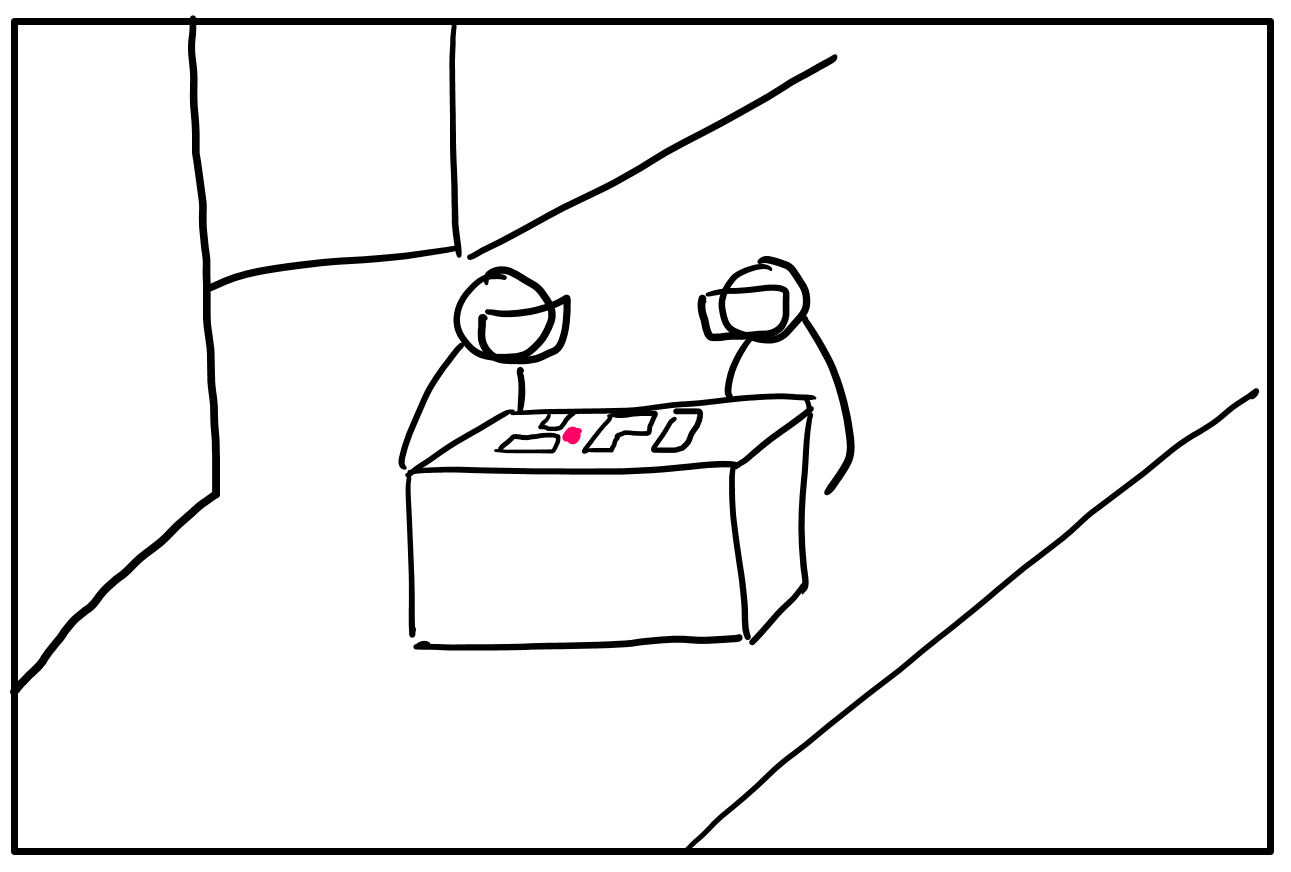
\includegraphics[scale=.2]{figures/comics/uncomfortable_collaboration.png}}
	\end{minipage}%
	\begin{minipage}{.25\linewidth}
		\centering
		\subfloat{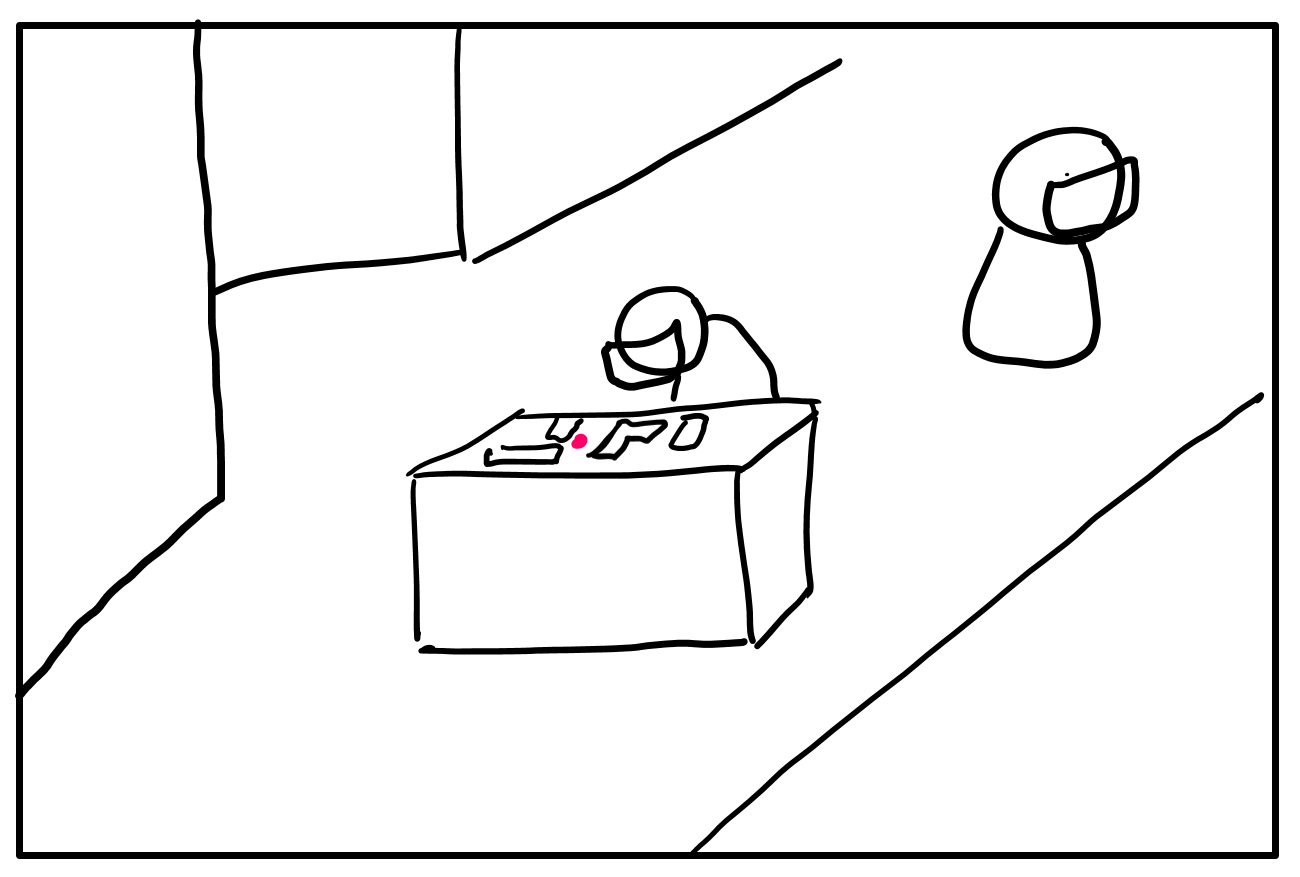
\includegraphics[scale=.2]{figures/comics/uncomfortable_collaboration2.png}}
	\end{minipage}%
	\begin{minipage}{.25\linewidth}
	\centering
	\subfloat{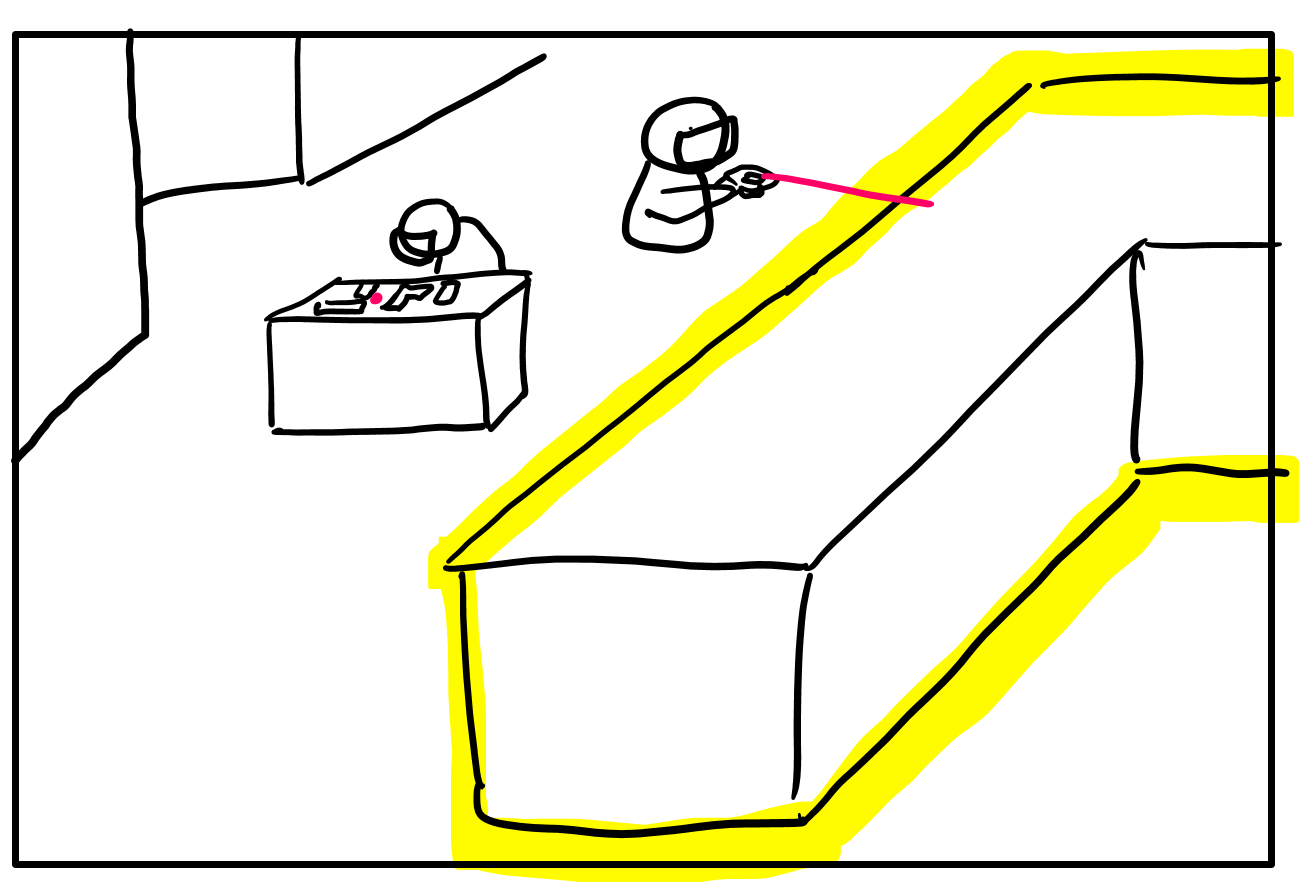
\includegraphics[scale=.2]{figures/comics/uncomfortable_collaboration3.png}}
	\end{minipage}
	
	\par\medskip
	\begin{minipage}{.25\linewidth}
		\centering
		\subfloat{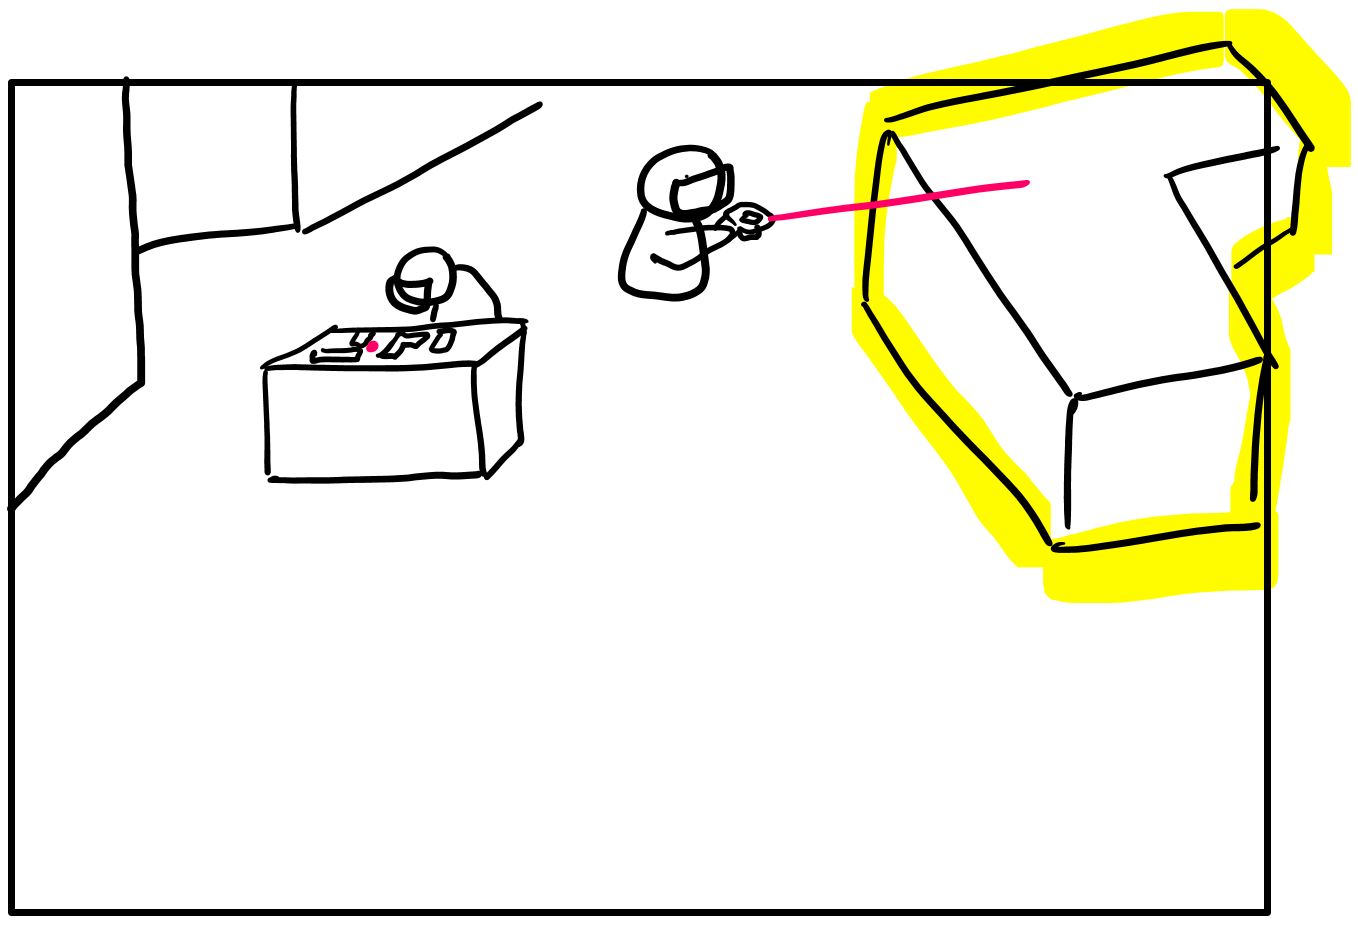
\includegraphics[scale=.2]{figures/comics/uncomfortable_collaboration4.png}}
	\end{minipage}%
	\begin{minipage}{.25\linewidth}
		\centering
		\subfloat{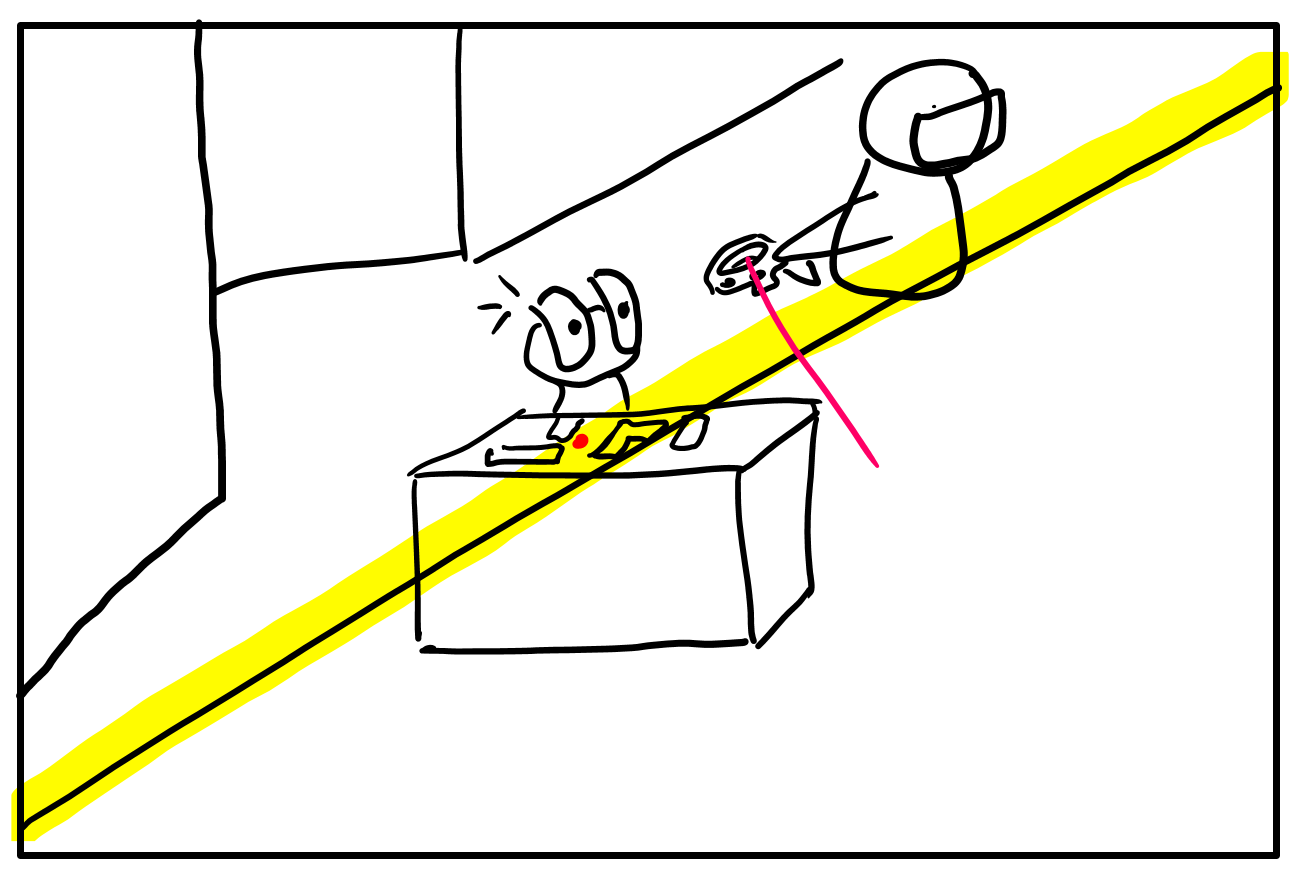
\includegraphics[scale=.2]{figures/comics/uncomfortable_collaboration5.png}}
	\end{minipage}%
	\begin{minipage}{.25\linewidth}
		\centering
		\subfloat{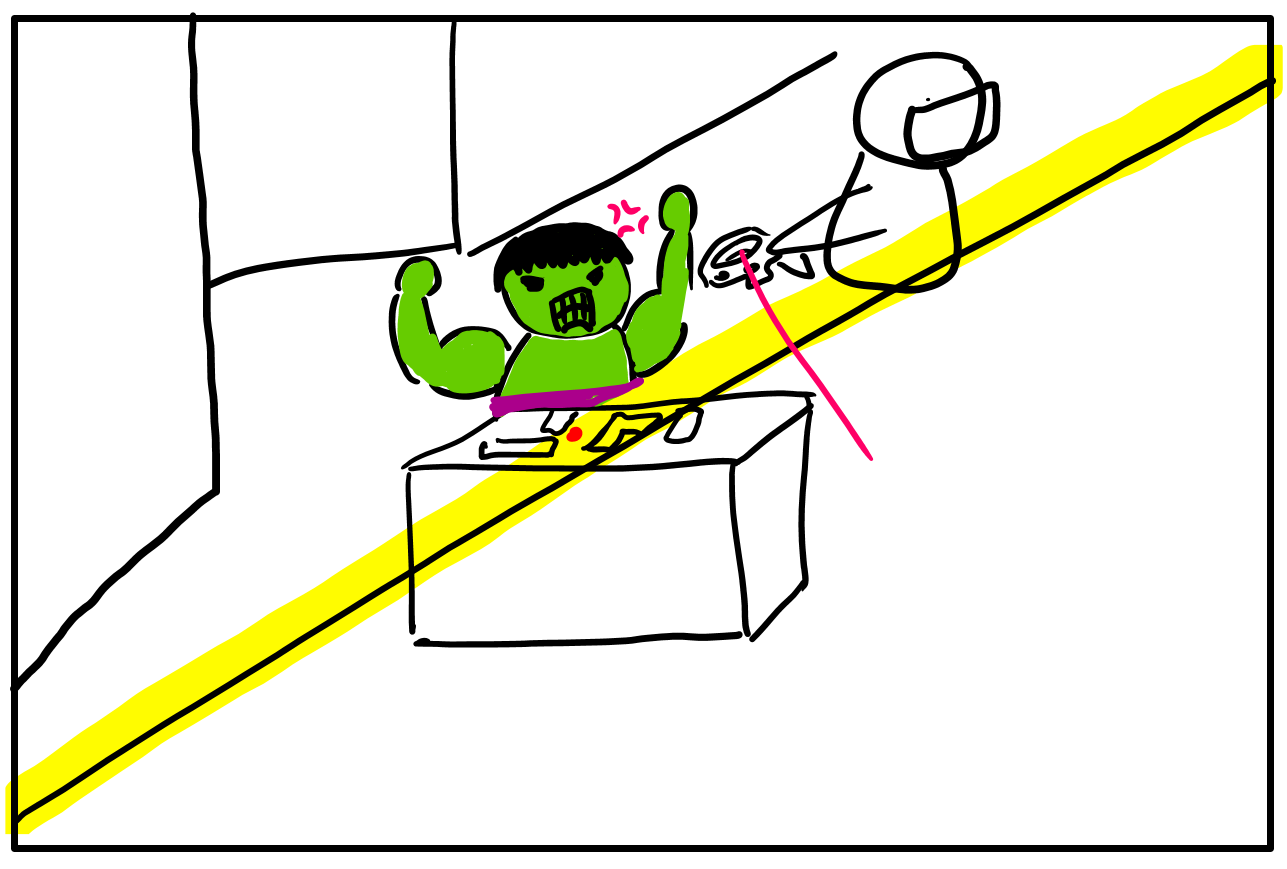
\includegraphics[scale=.2]{figures/comics/uncomfortable_collaboration6.png}}
	\end{minipage}
	
	\caption{Collaborators unaware of each other's actions}
	\label{fig:a1unawareofa2actions}
\end{figure}


%---------------Reference commands and structires

% \chapter{Introduction}\label{chapter:introduction}
% \section{Motivation: Teamwork is important. Creative thinking implies generation of ideas, collaboration, and communication. Virtual Reality (VR) is a great enhancement for creative thinking tool-set in architecture.}
%\subsection{Solution validation/evaluation in HCI: methods, and principles.}
\begin{comment}
Methodology: approach to solving the problem; chosen HCI methodology for the final evaluation - no idea
a. Chosen HCI evaluation methodology
\end{comment}


\begin{comment}
See~\autoref{tab:sample}, \autoref{fig:sample-drawing}, \autoref{fig:sample-plot}, \autoref{fig:sample-listing}.
\begin{table}[htpb]
  \caption[Example table]{An example for a simple table.}\label{tab:sample}
  \centering
  \begin{tabular}{l l l l}
    \toprule
      A & B & C & D \\
    \midrule
      1 & 2 & 1 & 2 \\
      2 & 3 & 2 & 3 \\
    \bottomrule
  \end{tabular}
\end{table}

\begin{figure}[htpb]
  \centering
  % This should probably go into a file in figures/
  \begin{tikzpicture}[node distance=3cm]
    \node (R0) {$R_1$};
    \node (R1) [right of=R0] {$R_2$};
    \node (R2) [below of=R1] {$R_4$};
    \node (R3) [below of=R0] {$R_3$};
    \node (R4) [right of=R1] {$R_5$};

    \path[every node]
      (R0) edge (R1)
      (R0) edge (R3)
      (R3) edge (R2)
      (R2) edge (R1)
      (R1) edge (R4);
  \end{tikzpicture}
  \caption[Example drawing]{An example for a simple drawing.}\label{fig:sample-drawing}
\end{figure}

\begin{figure}[htpb]
  \centering

  \pgfplotstableset{col sep=&, row sep=\\}
  % This should probably go into a file in data/
  \pgfplotstableread{
    a & b    \\
    1 & 1000 \\
    2 & 1500 \\
    3 & 1600 \\
  }\exampleA
  \pgfplotstableread{
    a & b    \\
    1 & 1200 \\
    2 & 800 \\
    3 & 1400 \\
  }\exampleB
  % This should probably go into a file in figures/
  \begin{tikzpicture}
    \begin{axis}[
        ymin=0,
        legend style={legend pos=south east},
        grid,
        thick,
        ylabel=Y,
        xlabel=X
      ]
      \addplot table[x=a, y=b]{\exampleA};
      \addlegendentry{Example A};
      \addplot table[x=a, y=b]{\exampleB};
      \addlegendentry{Example B};
    \end{axis}
  \end{tikzpicture}
  \caption[Example plot]{An example for a simple plot.}\label{fig:sample-plot}
\end{figure}

\begin{figure}[htpb]
  \centering
  \begin{tabular}{c}
  \begin{lstlisting}[language=SQL]
    SELECT * FROM tbl WHERE tbl.str = "str"
  \end{lstlisting}
  \end{tabular}
  \caption[Example listing]{An example for a source code listing.}\label{fig:sample-listing}
\end{figure}
\end{comment}